\label{chapter-scenario-template}
\textbf{Created by:} Perawit Charoenwut \\
\textbf{Modified by:}

\subsection*{Scenario Objective}
This scenario aims to demonstrate how to model relationships between different types of agents in commercial transactions using the IOF Core patterns. The pattern models how different entities (such as persons and organizations) can take on specific roles (such as buyer and supplier) within complementary business processes that involve material products. This pattern is fundamental for representing any transaction where one party acquires a product from another, making it clear which agents are involved and what their specific roles are within the transaction context.

\subsection*{General Pattern Description}
The pattern models the relationship between buyers, suppliers, and material products through their roles and participation in business processes. It demonstrates how:

An agent classified as a Buyer has a BuyerRole that participates in a BuyingBusinessProcess
An agent classified as a Supplier has a SupplierRole that participates in a SupplyingBusinessProcess
Both business processes have the same MaterialProduct as a participant

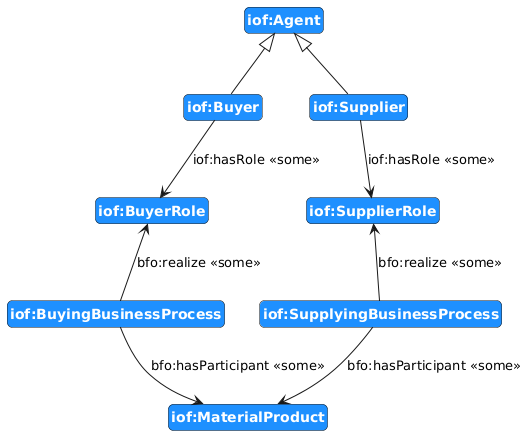
\includegraphics[scale=0.4]{scenarios/different-type-agent/image/different-type-agent-schema.png}

\subsection*{Use Case: Coffee Shop Transaction}
\subsubsection*{Use-Case Pattern Description}
This use case demonstrates how a buyer (John), purchases a cup of coffee from a cafe. 

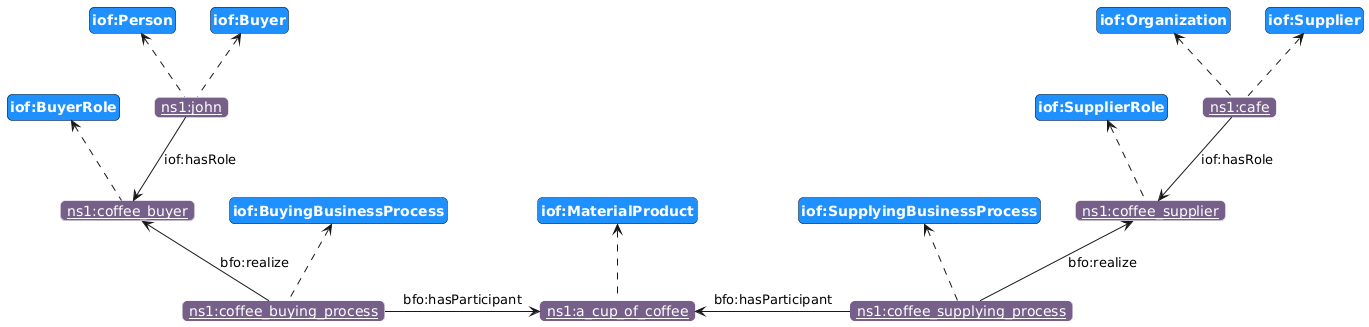
\includegraphics[scale=0.35]{scenarios/different-type-agent/image/different-type-agent.png}


\subsubsection*{Use-Case Example Data}


\begin{table}[h]
% \caption{}
\label{tab:organization-structure}
% \resizebox{\columnwidth}{!}{%
\begin{tabular}{|l|l|}
\hline

\hline
\end{tabular}%
% }
\end{table}


\subsubsection*{Data Mapping}
\begin{verbatim}

\end{verbatim}



\subsubsection*{Data Validation}
